% Compile with latex, not pdflatex (or pic circles wont show up)
% If there are problems with figures, remember they should be eps or pic
\documentclass[a4paper]{article}
\usepackage{graphicx}
\usepackage[utf8]{inputenc}
\title{title perhaps continued here with \texttt{verb \\} text}
\author{author info\\
more author info with \texttt{tt text}} 

\begin{document}

\maketitle{}
\begin{abstract}
A section perhaps with the abstract if it's titled "Abstract".

\end{abstract}
\section{A sect}
\label{sec1}
\subsection{A subsect}
\label{sec1x1}
Use \ref{sec1}, or any keys, to refer to the section with the title
containing all the words.

\subsubsection{A sub-sub sect}
\label{sec1x1x1}
.abc escaped

'abc escaped \_

"cd escaped"

\%tex comment scaped

some text making one paragraph\\
with a forced line break

\texttt{verb} at the start of a par.

another paragraph

\begin{itemize}
\item[]
    To relatively indent a paragraph, use the tab.

\end{itemize}
This executes a command and takes its output as verbatim text:
\begin{itemize}
\item[]
    \begin{verbatim}
    Wed Apr 29 16:34:34 CEST 2015
    Wed Apr 29 16:34:34 CEST 2015
    \end{verbatim}

\end{itemize}
yet another paragraph
\begin{itemize}
\item[]
    with closely indented par
\end{itemize}
within other text

this paragraph includes a list of items
\begin{itemize}

    \item item 1 starts here and continues with more text

    another paragrah within the same item, starting a new itemize
    \begin{itemize}

        \item 2nd level 1st item

        \item 2nd level 2nd item
    \end{itemize}

    \item item 2 text continued here

    \item item 3 text using multiple lines

\end{itemize}
after this paragraph comes some indented text with a list\\
of numbered items and another list of items.

\begin{itemize}
\item[]
    some indented text
\end{itemize}
\begin{enumerate}

    \item first numbered item

    \item another

    \item yet another
\end{enumerate}
\begin{itemize}

    \item first item

    \item last item

\end{itemize}
A description list is a list of items where each item ends within the
first line and is followed by indented paragraphs describing the item.
It is ok if the entire description name (item) is marked with a font
indicator, but items should be simple names and cannot have font
switches or other markups in the middle.
\begin{description}
    \item[\textit{first description}]
        for this and that

        with a second paragraph.

    \item[\texttt{/a/b/c}]
        for this other thing
    \item[-f]
        for another thing

\end{description}
this text has some \textbf{text set in bold face} and some in
\textit{italic}, and some in \texttt{teletype font}.

Within teletype font \texttt{no character is special, including \_
and *}. This is good for things like \texttt{/a/b/c}.

You can repeat the * to scape it, or \_ or |.

you can use\Large (or + any other number) to increase to a bigger
font size and\normalsize to return to the normal size, and you can
use
\textit{%
to italize a set of lines
}%
or start an
\begin{itemize}
\item[]
    indented paragraph and then
\textbf{%
    make a set of lines bold
}%
\end{itemize}
or
\texttt{%
make a set of lines fixed font
}%

this paragraph has
\begin{itemize}
\item[]
    \begin{verbatim}
    .text starting with dot
    some indented verbatim text, including ['s and ]'s and \n
    nb = 0
    [
        pf = pf.Close()
    ]
    wrelems(out, e.Child, lvl+1)
    \end{verbatim}
\end{itemize}
but the verbatim text could be unindented as well.

this other paragraph has a cite [for this] and a url for the lsub page
\verb|http://lsub.org| within the rest of the text you could also
place a link to \verb|http://google.com|. Imprecise citations like
\cite{bib1,bib2,bib2} can also be made.

    \begin{figure}
    \centering
        
\includegraphics[width=\linewidth]{logols.pdf}
    \label{fig1}
    \caption{Caption goes here and perhaps continues here. }
    \end{figure}

or write pic directly in place

\begin{figure}
\centering
    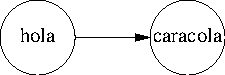
\includegraphics{/zx/sys/src/clive/app/wr/example_pic2.pdf}
\label{fig2}
\caption{the caption starts without indentation and may span several
lines. }
\end{figure}

Fig is number \ref{fig2}.

Use \ref{tbl1} for tables, \ref{eqn1} for eqns, and \ref{lstkey}
for listings. Do not use these references at the start of text in a
line or they may be understood as an actual table, etc.

for tables and equations we can use
\begin{table}
\centering
    \begin{tabular}{||l|c|r|}\hline
        	&col2	&col3\\ \hline
        row1	&11	&12\\ \hline
        row2	&21	&22\\
        \hline
    \end{tabular}
\label{tbl1}
    \caption{tables may have captions. The first line of items always
    describes column formats, the second line always describes columns,
    and the first column always describes rows. No other table formats are
    supported. }
\end{table}

\begin{figure}
\centering
    
\includegraphics{/zx/sys/src/clive/app/wr/example_eqn1.pdf}
\label{eqn1}
\caption{eqns may have captions }
\end{figure}

\begin{figure}
\centering
    \begin{verbatim}
        {
            some prog or code
            taken verbatim to be printed
        }

    \end{verbatim}
\label{lst1}
\caption{it may have caption, the word after [code is used as a tag
in the listing. the default is program. but all code listings share
the same code counter despite the tag used. You can use
\texttt{marks} and [cites] here. }
\end{figure}

and \$so on...
\begin{thebibliography}{50}
\bibitem{bib1}     The organization of networks in Plan 9. D. Presotto, P. Winterbottom.
    USENIX Association. Proceedings of the Winter 1993 USENIX Conference.
    1993.
\bibitem{bib2}     Plan B User's Manual. Second edition. Laboratorio de Systemas, URJC.
    GSYC-TR-2004-04. 2004.
\end{thebibliography}

\end{document}
